\chapter{Bayesian Optimization}
This chapter will introduce Bayesian optimization. We start with a general introduction to the
concept of optimization (mainly based on \cite{bayesoptbook}), which culminates with the
introduction of the idea of Bayesian optimization (BO). Next, we dive into the first BO component:
The Bayesian regression methodology. Finally, the concept of an acquisition function is introduced,
with a focus on expected improvement and a brief description of the other types. 

\section{Optimization methodology}
Given a cost/objective function $f: \mathcal{X} \rightarrow \mathbb{R}$, where the domain
$\mathcal{X}$ could be a subset of $\mathbb{R}^n$,
optimization is a methodology which seeks to find an optimal point, $x^*$, and value
$f^* = f(x)$, given as
\begin{align}\label{OPT}
    x^* \in \arg\min_{x \in \mathcal{X}} f(x) \hspace{1cm} f^* = \min_{x \in \mathcal{X}} f(x) = f(x^*).
\end{align}
Note that the above formulation is a minimization problem, which is equivalent to a
maximization problem maximizing $-f(\cdot)$. Throughout this thesis, we choose to only work
with a minimization problem. 
Solving this problem is intractable except for rare cases e.g. if $f$ is 
convex and analytically directly solvable or the domain of $f$ is very limited. Hm

\begin{testexample}[Direct solution method]
    The unconstrained linear least squares, $$\min_{x\in \mathbb{R}^n} f(x) := ||Ax-b||_2^2$$
    where $A \in \mathbb{R}^{m\times n}$ and $b \in \mathbb{R}^m$, is a convex problem,
    i.e. finding $x^*$ such that $\nabla f(x^*) = 0$ is equivalent to finding the solution
    to the problem. Assuming $A^TA$ is invertable, linear least squares can be solved
    directly by the normal equations, 
    $$\nabla f(x) = 2A^TAx + 2b^TA = 0 \hspace{0.5cm} \Leftrightarrow \hspace{0.5cm} x^* = (A^TA)^{-1} A^Tb$$
\end{testexample}

Most optimization problems are non-convex with multiple local minima. And even if the gradient is
given analytically the solution is found among a potentially infinitely large 
set of stationary points ($\nabla f(x) = 0$) and boundary points - this might be tedious or impossible.
When the problem is not directly solvable, mathematical optimization takes an indirect methodology: 
Design a sequence of experiments that reveal information of the objective function. This information 
can hopefully lead us to the solution of \eqref{OPT}. This general way of sequentially solving 
is presented in the book Bayesian Optimization by Roman Garnett \cite{bayesoptbook} and 
presented here as Algorithm \ref{algOPT}. 
W
\begin{algorithm}
\caption{Sequencial Optimization \cite{bayesoptbook} }\label{algOPT}
\begin{algorithmic}
\State \textbf{Input:} Initial dataset $\mathcal{D}$  \Comment{can be empty}
\While{Temination is not reached}
    \State $x \gets \text{policy}(\mathcal{D})$ \Comment{select next observation location}
    \State $y \gets \text{observe}(x)$ \Comment{observe objective function at chosen location}
    \State $\mathcal{D} \gets \mathcal{D} \cup \{(x,y)\} $ \Comment{update dataset}
\EndWhile
\State $\textbf{return: } \mathcal{D}$
\end{algorithmic}
\end{algorithm}

Given data points in the optimization landscape\footnote{"Optimization landscape" defined as the joint set of points in the domain and the objective function
evaluated in the points, i.e. $\{(x,f(x))\in \mathcal{X} \times \mathbb{R}| x \in \mathcal{X}\}$} 
a policy selects a point $x \in \mathcal{X}$ where we make our next observation. Policies can be deterministic or probibalitic, e.g. 
grid search and random search are examples of policies. The next observation provides us a $y$ value, which combined with $x$ is included to the 
available data $\mathcal{D}$. Finaly, a stopping criterion decides whether to continue or terminate. 

<example of random search is half as efficient as BO>


\begin{testexample}[Grid search]
    In grid search values along each dimention in $\mathcal{X}$ is seleced and combined with each
    other, which thereby defines a grid in the parameter space. All points are ordered and systematicly
    selected. In the content of algorhtim \ref{algOPT} we define the grid search policy as 
    $$\text{policy}_{GS}(\mathcal{D}) = x_{|\mathcal{D}|+1}$$
    assuming $x_1,x_2, \dots, x_{n}$ are the ordered grid points and the size of the obtained 
    data is $|\mathcal{D}|$. 
\end{testexample}
\begin{testexample}[Random search]
    In random search a uniform distribtuion is layed over the domain space $\mathcal{X}$ and a random point
    is selected from the distribtuion. 
    $$\text{policy}_{RS}(\mathcal{D}) = x, \hspace{0.5cm} x \sim p(\mathcal{X})$$
    Note that grid search and random search are policies which completely 
    ignores the available data. This is a shame and we can do better. 
\end{testexample}

\begin{testexample}[Gradient descent]
    Gradient descent is the most simple gradient-based optimization approach. The gradient of a continuous 
    function points in the most ascending direction from the location where it is evaluated.
    In the minimization task, \eqref{OPT}, we can iteratively use the opposite gradient direction, i.e. the most 
    descenting directiong. This yields the policy:
    $$\text{policy}_{GD}(\mathcal{D}) = x_n - \eta \nabla f(x_n)$$
    where we for a brief moment modify $y$ to be a vector, since the observation model 
    is given as:
    $$\text{observe}_{GD}(x) = [f(x), \nabla f(x)]$$
\end{testexample}

\begin{testexample}[Surrogate-based optimization]
    <SVR> <Radial Basis function> <Polynomal model/respons surface>
    In surrogate-based optimization all available data is fitted by a cheap-to-evaluate approximation
    to the objective function - this approximation is called a \textit{surrogate} model. Examples
    of surrogate models could be a neural network or a random forest. The next point is 
    chosen as the point where the surrogate model is minimized. 
    $$\text{policy}_{sur}(\mathcal{D}) = \min_x \hat f(x)$$
    where $\hat f(x) \approx f(x)$ for $x$ close to the data $\mathcal{D}$. And we hope the approximation
    holds for $x$ far away from the the data. \textbf{}
\end{testexample}

\subsection{When to use Bayesian optmization}
What if $f(x)$ took serval days to evaluate. What if $f(x)$ is noisy? what if discrete points? 
<more here>

% \begin{figure}[h]
%     \centering
%     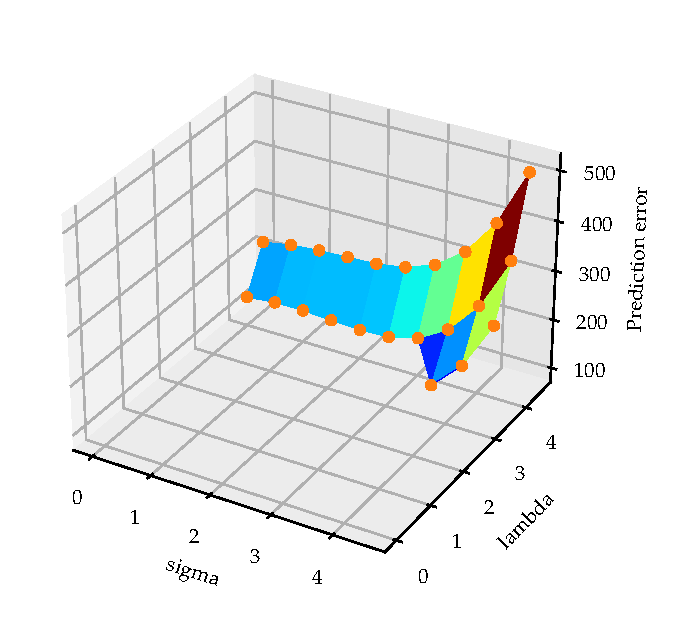
\includegraphics[width=0.9\textwidth]{Pictures/BO_vs_Grid2.eps}
%     \caption{Hyper parameter tuning of a model $M(\lambda, \sigma)$, 
%     35 evaluation in grid search vs 39 evaluations using Bayesian optimization}
%     \label{optimhist}
% \end{figure}
\begin{tcolorbox}[
    sharp corners,
    boxrule=0mm,
    enhanced,
    borderline west={4pt}{0pt}{gray},
    colframe=drGray,
    colback=drGray,
    coltitle=black,
]
{\large \textbf{Example: Bayesian Optimization}}\\
    Bayesian optimization is a \textit{probabilistic} surrogate-based optimization
    methodology. Here a cheap probabilistic regression model $p(y|x)$ is fitted to the
    the observations $\mathcal{D}$ and oppose to (deterministic) surrogate-based
    optimization, it is not possible right away to find the minima in the cheap
    surrogate model; first, we need to interpret the meaning of minima in a probabilistic
    regression model. This interpretation is done through a so-called acquisition
    function (more about this later). The policy is as following,
    $$\text{policy}_{BO}(\mathcal{D}) = \max_x AQ(p(y|x))$$
\end{tcolorbox}
\begin{figure}[H]%
    \centering
    {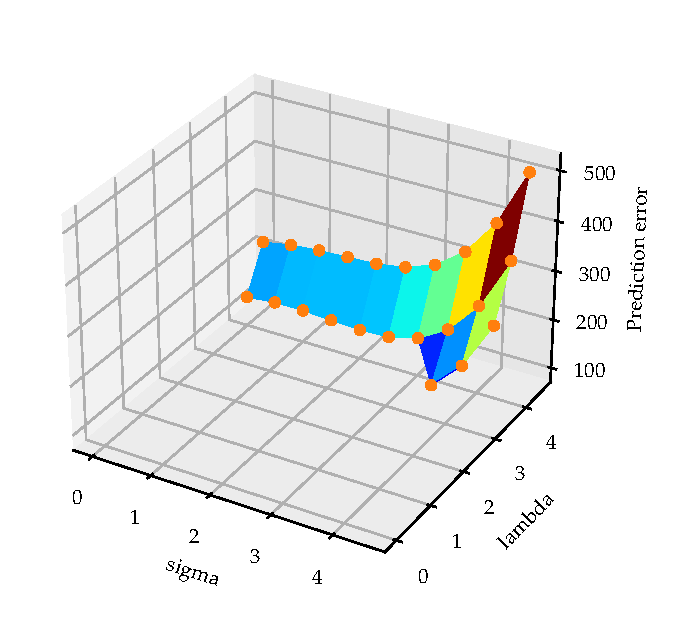
\includegraphics[width=0.46\textwidth]{Pictures/BO_vs_Grid2.eps} }%
    \qquad
   {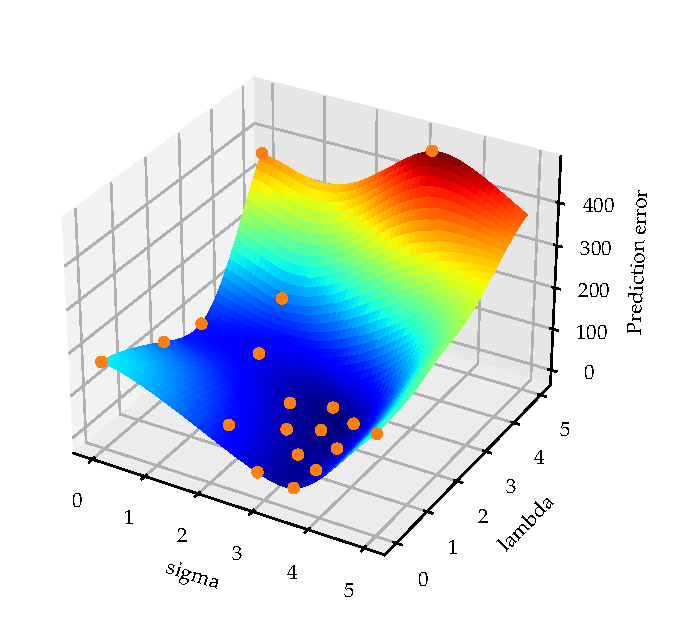
\includegraphics[width=0.46\textwidth]{Pictures/BO_vs_Grid1.eps} }%
    \caption{Hyper parameter tuning of a model $M(\lambda, \sigma)$, 
    23 evaluation in grid search vs 23 evaluations using Bayesian optimization}%
    \label{fig:example}%
\end{figure}


additionally, Bayesian Optimization allow for observation noise, 

\subsection{Observation model}\label{ObsModel}
Many optimization algorithms assume \textit{exact} evaluations of the objective function. However, this assumption
is often wrong especially for objective functions with real-life experiments, imperfect simulations, human interaction 
where measurement noise is a well known. The observation model is typically noisy and described as
$$y = f(x)+\epsilon$$ where $\epsilon$ is the measurement error, this is
typically assumed to be Gaussian with zero mean and a variance
$\sigma^2$ (which could depend on $x$ in a heterostodatic setting) and implies a Gaussian observation model, 
$$p(y|x,f(x),\sigma) = \mathcal{N}(y;f(x),\sigma^2)$$ 

% (note from now on we define $\phi := f(x)$ in order to avoid confusion and a extra set of paranteses)
% $$p(y|x,\phi,\sigma) = \mathcal{N}(y;\phi,\sigma^2)$$ 
we can extend this model to deal with noiseless observations as well, simply by setting $\sigma = 0$ and let the
model colaps into a Direct delta distribution, 
$$p(y|x, f(x)) = \mathcal{\delta}(y-f(x))$$
i.e. all probability mass for $y$ is on the value $f(x)$ giving the observation sample $y = f(x)$




% <Cope with inacuracies> i.e. allows for stochastic objective function. 
% <Uncertainty measure with prediction based on simple and clear prior 
% assumptions about the characteristic about the objective function. >
% <Provides an adequate termination condition for the opt. process>. 

% <kilde 151. Bayes Opt is assumed superior to other global optimization technics 
% with limited budget>

\section{Bayesian regression}
% \begin{testexample2}[Bayesian methodology]
%     In Bayesian statistics $p(\theta|\mathcal{D})$ is the posterior distribution, and it is 
% of $\theta$ is linked to the likelihood and prior via Bayes rule,
% $$p(\theta|\mathcal{D}) = \frac{p(\mathcal{D}|\theta)p(\theta)}{p(\mathcal{D})}$$
% \end{testexample2}
Whereas traditional regression workflow is the following: Given data, choose the best fitting model
parameters, make predictions using those parameters. The Bayesian framework allows us to skip the
dependency of a single set of parameters and instead use \textit{all possible} parameters by treating the set
of parameters as a random quantity, $\theta \sim p(\theta|\mathcal{D})$, where some values/realizations of $\theta$ are more
probable than others given data. In Bayesian regression we are interest is the predictive posterior distribution,  
\begin{align}\label{Predictive2}
    p(y|x, \mathcal{D}) &= \int p(y,\theta|x, \mathcal{D}) d\theta\\
    &= \int p(y|x,\theta)p(\theta|\mathcal{D}) d\theta,
\end{align}
where the posterior $p(\theta|\mathcal{D})$ gives weighting to the proposed regression model
$p(y|x,\theta)$. Note that the second equation is true because of the probability chain rule and
that $y$ is fully described by the parametric model $p(y|x,\theta)$ and the parameters $\theta$ are
fully described by the posterior distribution $p(\theta|\mathcal{D})$.


\subsection{Surrogate model}
A surrogate model in a Bayesian optimization setting is a Bayesian regression model. The most
used surrogate model is a Gaussian Process. But there have been investigations on other 
surrogates, such as Bayesian neural networks and Bayesian regression trees. These are all
discriminative models, and another approach we focus on in this project is to model $y$ and
$x$ jointly in a so-called generative model, $p(x,y)$. A generative model can be used implicitly
as a surrogate from the conditional distribution of $y$ given $x$, $p(y|x)$.

In this thesis, the Bayesian regression models investigated as Bayesian optimization surrogates are
the following:
\begin{itemize}[noitemsep]
    \item Gaussian process (GP)
    \item Bayesian neural network (BNN)
    \item Kernel density regression (KDE)
    \item Gaussian mixture regression (GMR)
    \item Sum-product networks (SPN)
\end{itemize}

We now introduce the concept of inference, which is necessary for using the probabilistic surrogate models
in Bayesian Optimization. 

\subsection{Inference of surrogate models}
Inference is the process of computing answers to queries about a probabilistic model after observing
data. In Bayesian regression, the query is the predictive distribution, $p(y|x,\mathcal{D})$, as we
are interested in the distribution of $y$ given $x$ and already observed data, $\mathcal{D}$. This
often indirectly create the posterior query, $p(\theta|\mathcal{D})$, the probability of model
parameters $\theta$ given data $\mathcal{D}$. Lastly, it is also inference when we train a Gaussian
mixture model or SPN using the expectation-maximization algorithm (EM) since we are iteratively
answering the query $E_{p(z|\theta^{(k)})}[z|\theta]$.

%\subsection{Exact and approximate inference}
We distinguish between two different ways of inference: Exact and approximate inference. It is
\textit{exact inference} when a probabilistic query is calculated exact. It is possible to
calculate exact inference on the predictive distribution for the Gaussian mixture model, Sum product
network, and Gaussian processes. Models which allow for exact inference have a powerful advantage
over the models with approximate inference since we can guarantee the answers to the queries are
correct; however, they are usually also less expressive (unable to explain complicated models). 

When it is not possible to answer a probabilistic query exact, we can approximate the answer using
\textit{approximate inference}. When dealing with complicated and expressive statistical models,
exact inference is often intractable, and we need to use approximate inference. Approximate
inference is a broad category of methods, which includes variational inference and Markov chain
Monte Carlo (MCMC). The two Bayesian Neural networks, we deal with in this project, Bohamiann and
Numpyro BNN are similar regression models but are inferred using two different MCMC methods,
Hamiltonian Monte Carlo - giving different results. As revealed later (see in section \ref{BNN})
approximate inference might be flawed and inexact. 

\begin{table}[H]
    \centering
    \begin{tabular}{l|l|l}
    %\rowcolor[HTML]{C0C0C0} 
    \textbf{Model}       & \textbf{Predictive inference}    &   \textbf{Learning} \\ \hline
    GP                          & Exact $O(n^3)$            & Emperical Bayes\\
    Numpyro BNN                 & No U-Turn Sampler         & \\
    Bohamiann BNN               & Adaptive stochatic HMC    & \\
    Kernel density regression   & Exact $O(n)$              & \\
    Gaussian mixture regression & Exact $O(K)$              & EM  \\
    SPN                         & Exact $O(E)$              &  EM $O(E)$\\
    \end{tabular}
    \caption{Overview of inference methods applied on the statistical models used in this project.
            $E$ is the number of edges in the SPN. $n$ is the number of data points. $K \leq n$ is
            the number of mixture components. We will soon learn that for an SPN the number of
            mixture components is exponentially larger than the number of edges i.e. $E << K$. In theory
            MCMC methods samples from true the posterior distribution, and do not need any
            fitting/learning. }
\end{table}

\newpage
\section{Acquisition function}
Given a correct predictive distribution $p(y|x\mathcal{D})$ the next step in Bayesian optimization
is to select the next location $x \in \mathcal{X}$ to sample from. The next location is chosen
according to a so-called acquisition function (AQ function), which balances out the well-known
concept of exploitation and exploration. It is exploitation if the next chosen location according to
its average improvement. It is exploration if the next point is chosen in a region of high
uncertainty and thereby helps lower the overall uncertainty. First, we will look at the acquisition
function used in the thesis: Expected improvement. Secondly, we shortly present other different
types of acquisition functions. In Figure \ref{Different_AQ_functions} we see three different
acquisition functions. The expected improvement (EI) is known for being biased towards exploitation.
In contrast, the negative lower confidence bound (LCB) has a parameter $\beta$, which can be tuned
to make it focus more on exploration. 
\begin{figure}[H]
    \centering
    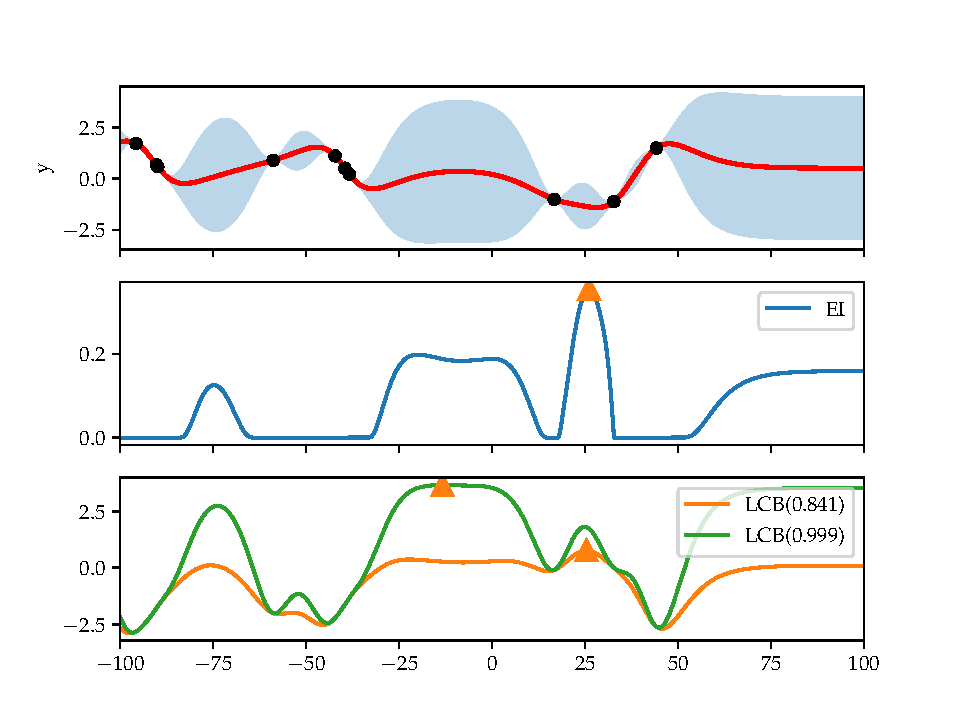
\includegraphics[trim=1cm 0cm 1cm 1cm,clip,width=\textwidth]{Pictures/illustration_AQs.pdf}
    \caption{The same regression model and points as Figure \ref{BO_example}, but with three
    different acquisition functions: Expected improvement and negative lower confidence bound for
    two different lower quantiles $0.841$ and $0.999$. The latter yields more exploration.}\label{Different_AQ_functions}
\end{figure}

\begin{figure}[H]
    \centering
    \begin{minipage}[b]{0.32\textwidth}
      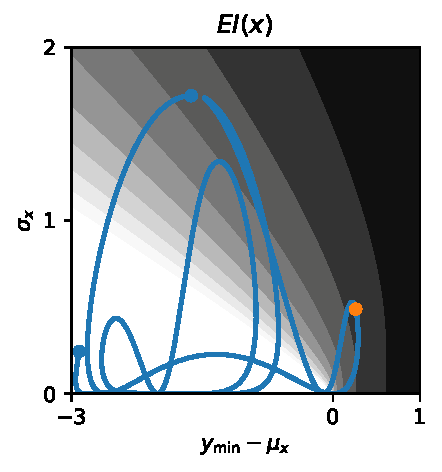
\includegraphics[trim=0.2cm 0.2cm 0cm 0.1cm,clip,width=\textwidth]{Pictures/expected_improvement_illustration.pdf}
    \end{minipage}
    \hfill
    \begin{minipage}[b]{0.32\textwidth}
        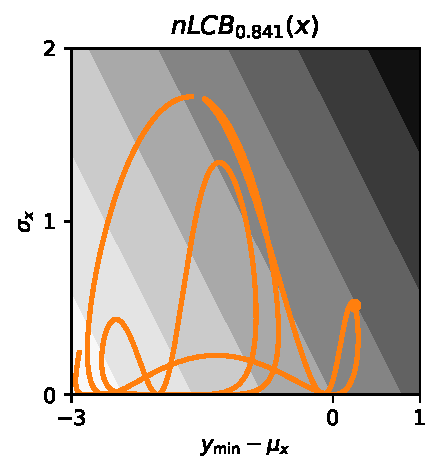
\includegraphics[trim=0.2cm 0.2cm 0cm 0.1cm,clip,width=\textwidth]{Pictures/neg_lower_confidence_illustration_1.pdf}
      \end{minipage}
     \hfill
     \begin{minipage}[b]{0.32\textwidth}
        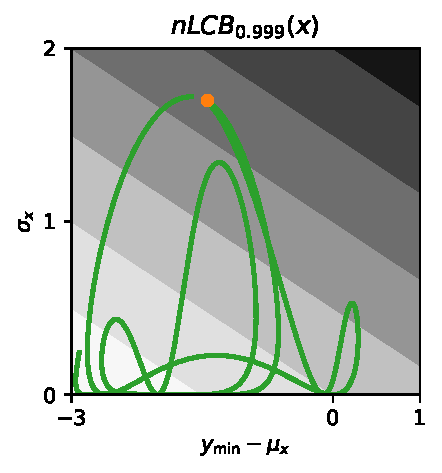
\includegraphics[trim=0.2cm 0.2cm 0cm 0.1cm,clip,width=\textwidth]{Pictures/neg_lower_confidence_illustration_3.pdf}
      \end{minipage}
    \caption{Contourplot of expected improvement and lower confidence bound (for two different
    quantiles) for different (Gaussian) predictive uncertainties $\sigma_x =
    \sqrt{\mathbb{V}ar_{p(y|x,\mathcal{D})y]}}$ versus the average improvement $y_{\min}-\mu_x$,
    where $\mu_x = E_{p(y|x,\mathcal{D})}[y]$ (high values are dark). The colored lines are the
    mapping $x \mapsto (\sigma_x, y_{\min}-\mu_x)$ for $x = [-100, 100]$ for the Bayesian regression
    function in Figure \ref{Different_AQ_functions} - and thereby explains how the acquisition
    functions balances exploitation and exploration. The orange dot represent the point maximizing
    the acquisition function}
    \label{EI_illustration}
\end{figure}


\subsection{Expected improvement}
A popular choice of acquisition function is expected improvement, 
$$EI(x) = \mathbb{E}_{p(y|x,\mathcal{D})}[\max(0, y_{\min}-y)]$$ where we only consider the values
$y$, which improves the current best value in the expectation of the predictive distribution,
$p(y|x,\mathcal{D})$. Therefore, a $x$ which yield a bad predictive mean value
$\mathbb{E}_{p(y|x,\mathcal{D})}[y]> y_{\min}$ might still be maximizing the expectated improvement,
if the predictive uncertainty is very large at $x$. Figure \ref{EI_illustration} illustrates that a
large uncertainty in the predictive distribution (represented as the predictive variance) can lead
to relative large values even for non-improving mean predictions.


\begin{note2}[Why defining expected improvment with max]    
    Note that $\max(0,\cdot)$ is important since the Bayesian optimization othervise reduces to
    a simple non-probabilistic surrogate-based optimization method,
    \begin{align*}
        \mathbb{E}_{p(y|x,\mathcal{D})}[y_{\min}-y] = y_{\min} - \mathbb{E}_{p(y|x,\mathcal{D})}[y]
    \end{align*}
    i.e. maximizing the above is equivalent to maximizing the predictive mean, and thereby we loose
    all the valuable information about the predictive uncertainties from the Bayesian regression model. 
\end{note2}

\subsubsection{Exact expected improvement} \label{ExactEI} 
In the following derivation we assume the
predictive distribution can be approxiamted by a normal distribution dependent on the point of
interest $x$ and the data $\mathcal{D}$ (note for the GP it is in fact not an approximation), 
$$p(y|x,\mathcal{D}) \approx \mathcal{N}(y|\mu(x,\mathcal{D}), \sigma^2(x,\mathcal{D}))$$ where we
will change to a less clumpsy notation $\mathcal{N}(y|\mu_x,
\sigma^2_x):=\mathcal{N}(y|\mu(x,\mathcal{D}), \sigma^2(x,\mathcal{D}))$. This is completely fine
since we $x$ is fixed (and $\mathcal{D}$ is fixed) when evaluating the expected improvement in a point
$x$. %  $\sigma_x := \sigma^2(x,\mathcal{D})$ and $\mu_x := \mu(x,\mathcal{D})$
%as evaluated functions, i.e. numbers. 
Furthermore, the density of
a standard normal distribution is denoted $\phi(\cdot):=\mathcal{N}(\cdot | 0,1)$, and the cumlative
density function (CDF) of a standard normal distribution is denoted, $\Phi(\cdot) :=
\int_{-\infty}^{\cdot} \phi(\epsilon)d\epsilon$. We will now see that the normal approximation
of the predictive distribution yiels closed form solution to the expected improvement function, 

\begin{align*}
    E_{\mathcal{N}(y|\mu_x, \sigma_x^2)}[\max(0,y_{\min}-y)] &= \int \max(0,y_{\min}-y) \mathcal{N}(y|\mu_x, \sigma_x^2) dy\\
    &= \int_{-\infty}^{y_{\min}} (y_{\min}-y) \frac{1}{\sigma_x}\phi\left(\frac{y-\mu_x}{\sigma_x}\right) dy\\
    &= \int_{-\infty}^{\frac{y_{\min}-\mu_x}{\sigma_x}} (y_{\min}-\mu_x-\sigma_x\epsilon) \frac{1}{\sigma_x}\phi\left(\epsilon\right) \sigma_x d\epsilon\\
    &= \int_{-\infty}^u \sigma_x \cdot (u-\epsilon) \phi(\epsilon) d\epsilon\\
    &=  \sigma_x \cdot \left( u\cdot \int_{-\infty}^u \phi(\epsilon) d\epsilon +\int_{-\infty}^u (-\epsilon)  \phi(\epsilon) d\epsilon \right) \\
    &= \sigma_x [u\Phi(u)+ \phi(u)]
\end{align*}

where $u:=\frac{y_{\min}-\mu_x}{\sigma_x}$. 

\begin{note2}[Derivation details]
    To understand the identity $\phi(u) = \int_{-\infty}^u
    (-\epsilon)  \phi(\epsilon) d\epsilon$ used in the last equality, we first see that the antiderivative
is $\phi(\epsilon) = \frac{1}{\sqrt{2\pi}} \exp\left(\frac{-\epsilon^2}{2}\right)$,
\begin{align*}
    \frac{d}{d \epsilon} \phi(\epsilon) =  \frac{1}{\sqrt{2\pi}}\frac{d}{d \epsilon}  \exp\left(\frac{-\epsilon^2}{2}\right) 
    =  \frac{1}{\sqrt{2\pi}}\exp\left(\frac{-\epsilon^2}{2}\right)(-\epsilon)
    = -\epsilon \phi(\epsilon)
\end{align*}
and evaluating the rieman integral is equivalent to evaluate the antiderivative in its boundaries, giving the 
solution, 
$$\int_{-\infty}^u
(-\epsilon)  \phi(\epsilon) d\epsilon = \left[\phi(\epsilon)\right]_{-\infty}^u = \phi(u)-0 = \phi(u)$$ 
\end{note2}

We can also explicily write the expected improvement as, 
$$EI(x) = (y_{\min}-\mu_x)\Phi\left(\frac{y_{\min}-\mu_x}{\sigma_x}\right)+ \sigma_x
\phi\left(\frac{y_{\min}-\mu_x}{\sigma_x}\right)$$ where the first part can be interpretted as
exploitation (favouring points with a large average improvement $I(x) := (y_{\min}-\mu_x)$) and the second
part can be seen a exploitation (favouring points with high uncertainty.). This can also be seen
in Figure \eqref{EI_illustration}, where it is clear that the expected improvement is growing for
growing average improvement $I(x)$ and also for growing prediction uncertainty $\sigma_x$.


% taking the derivative with
% respect to $I(x) := (y_{\min}-\mu_x)$ and $\sigma_x$, we see that expected improvement is is
% increasing if the improvement grows or if the variance $\sigma_x$ grows, i.e
% $$\frac{\partial EI(x)}{\partial I(x)} = \Phi\left(\frac{y_{\min}-\mu_x}{\sigma_x}\right) > 0, \hspace*{0.5cm} 
% \frac{\partial EI(x)}{\partial \sigma_x} = \phi\left(\frac{y_{\min}-\mu_x}{\sigma_x}\right) >0$$ 
% <obs mistake in the book!!!?>

\subsubsection{Approximate expected improvement}
If the predictive distribution is non-Gaussian, it is either possible to approximate it as a Gaussian
(By using the mean and variance of the predictive distribution to define the Gaussian approximation)
or calculate the expected improvement approximately as follows, 
\begin{align*}
    E_{p(y|x,\mathcal{D})}[\max(0,y_{\min}-y)] &= \int \max(0,y_{\min}-y) p(y|x,\mathcal{D}) dy\\
    &\approx \frac{1}{K} \sum_{k=1}^K  \max(0,y_{\min}-y^{(k)})
\end{align*}
where $y^{(k)}$ are samples from the predictive distribution.

% In the case of a parametric model
% like a Bayesian NN, then we already got posterior samples from posterior $\theta^{(k)} \sim p(\theta | \mathcal{D})$, giving, 
% $$p(y|x,\mathcal{D}) \approx \frac{1}{K_2} \sum_{k=1}^{K_2} p(y|x,\theta^{(k)})$$ where
% $p(y|x,\mathcal{D} = \mathcal{N}(y|NN_w,\sigma))$. So essentially we should sample from a sampled
% distribution, but instead the PhD thesis \cite{PhDthesis}, just sample the mean and set $K_2 = 1$... 


% \begin{align*}
%     \mathbb{E}_{y_*|\textbf{x}_*,D_n}[\max(0,y_{\min}-y_*)] &= ??\\
%     \mathbb{E}[\min(0,y_{\min}-y_*)|\textbf{x}_*,D_n] &= \int_{-\infty}^\infty \min(0,y_{\min}-y_*) p(y_*|\textbf{x}_*,D_n) dy_*\\
%     &= \int_{-\infty}^{y_{\min}} (y_{\min}-y_*) p(y_*|\textbf{x}_*,D_n) dy_*\\
%     &\approx \frac{1}{N} \sum_{\theta \in \Omega } [y_{\min}-f_\theta(x)]
% \end{align*}

% where $\Omega = \{\theta|f_{\theta}(x)< y_{\min}\}$

%\section{uncertainties}
%Alatoric vs epistemic uncertainties 

\subsection{Lower confidense bound}
Lower confidence bound is defined by a confidence paramter $\pi \in [0,1]$
and then the lower quantile $\int_{\infty}^x p(y|x,\mathcal{D})dy = (1-\pi)$
is chosen as the acquisition. For a Gaussian predictive distribution this is 
simply  <more..>
$$nLCB(x) = - (\mu_x - \beta \sigma_x)$$
where $\beta = \Phi^{-1}(1-\pi)$.  
% \begin{figure}[H]
%     \centering
%     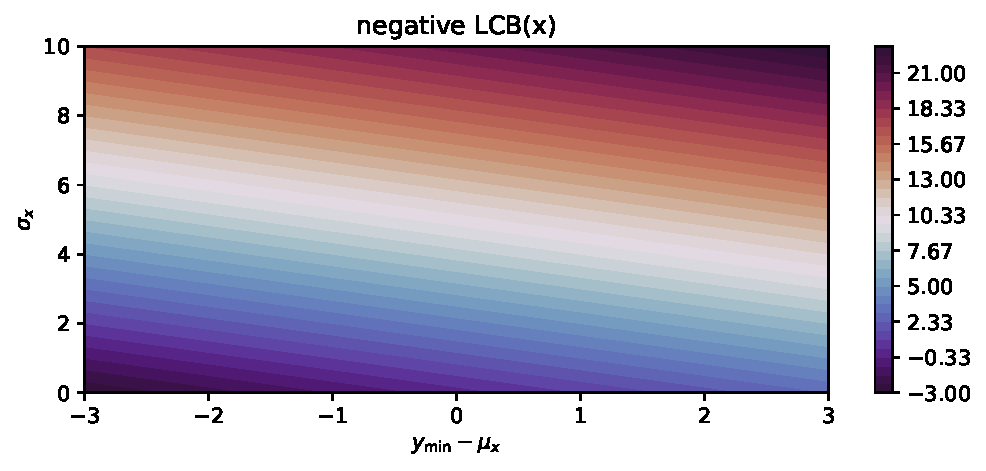
\includegraphics[width=\textwidth]{Pictures/neg_lower_confidence_illustration.pdf}
%     \caption{<Soon similar plot as Figure \ref{EI_illustration}> Illustration of the values of the
%     negative lower confidence bound for different predictive uncertainties $\sigma_x =
%     \sqrt{\mathbb{V}ar_{p(y|x,\mathcal{D})}[y]}$ versus the average improvement $y_{\min}-\mu_x$,
%     where $\mu_x = E_{p(y|x,\mathcal{D})}[y]$}
%     \label{nLCB_illustration}
% \end{figure}

\subsection{Entropy search}

<copy> An information theoretic approach
which accounts for the overall information gain on the optimizer ob-
tained from a new evaluation has also been presented. This is known
as informational approach to global optimization (IAGO), and uses en-
tropy as a measure for information (Villemonteix, Vazquez, and Walter,
2009).

\subsection{probability of improvement}


% We then discuss the knowledge
% gradient (Section 4.2), entropy search, and predictive entropy search (Section 4.3) acquisition functions.
% These alternate acquisition functions are most useful in exotic problems where an assumption made by
% expected improvement that the primary benefit of sampling occurs through an improvement at the point
% sampled is no longer true.


% The entropy search (ES) (Hennig and Schuler, 2012) acquisition function values the information we have
% about the location of the global maximum according to its differential entropy

% ES seeks the point to evaluate what causes the largest decrease in differential entropy

% (Recall from, e.g., Cover and Thomas (2012),
% that the differential entropy of a continuous probability distribution p(x) is R
% p(x) log(p(x)) dx, and that
% smaller differential entropy indicates less uncertainty.)

% Predictive entropy search (PES) (Hern´andezLobato et al., 2014) seeks the same point but uses a reformulation of the entropy reduction objective
% based on mutual information. Exact calculations of PES and ES would give equivalent acquisition functions, but exact calculation is not typically possible, and so the difference in computational techniques
% used to approximate the PES and ES acquisition functions creates practical differences in the sampling
% decisions that result from the two approaches. We first discuss ES and then PES.

% Let x  be the global optimum of f. The posterior distribution on f at time n induces a probability
% distribution for x
% . Indeed, if domain A were finite, we could represent f over its domain by a
% vector (f(x): x ∈ A), and x
% would correspond to the largest element in this vector. The distribution of
% this vector under the time-n posterior distribution would be multivariate normal, and this multivariate
% normal distribution would imply the distribution of x

% . When A is continuous, the same ideas apply,
% where x

% is a random variable whose distribution is implied by the Gaussian process posterior on f




% With kriging, we can develop search methods that put some emphasis on sampling where the standard
% error is high. In this way, we obtain the desired feature of ‘paying attention to parts of the space
% that have been relatively unexplored.’